\chapter{Аналитическая часть}


\section{Задача коммивояжёра}

\textit{Коммивояжёр} (фр. commis voyageur) -- бродячий торговец.

\textit{Задача коммивояжёра} -- важная задача транспортной логистики,
отрасли, занимающейся планированием транспортных перевозок.
Коммивояжёру, чтобы распродать нужные и не очень нужные в хозяйстве товары,
следует объехать n пунктов и в конце концов вернуться в исходный пункт.
Требуется определить наиболее выгодный маршрут объезда.
В качестве меры выгодности маршрута (точнее говоря, невыгодности)
может служить суммарное время в пути, суммарная стоимость дороги, или,
в простейшем случае, длина маршрута.



\section{Решение полным перебором}

Задача может быть решена перебором всех вариантов объезда и выбором оптимального.
Но при таком подходе количество возможных маршрутов очень
быстро возрастает с ростом n (оно равно n! — количеству способов упорядочения пунктов).
К примеру, для 100 пунктов количество вариантов будет представляться 158-значным числом.
Мощная ЭВМ, способная перебирать миллион вариантов в секунду,
будет решать такую задачу на протяжении примерно 3*10144 лет.
Увеличение производительности ЭВМ в 1000 раз даст хоть и меньшее в 1000 раз,
но по-прежнему очень большое время перебора вариантов.

Хотя такой подход и гарантирует точное решение задачи,
уже при небольшом числе городов решение за допустимое количество времени невозможно.


\section{Решение с помощью муравьиного алгоритма}

В то время как простой метод перебора всех вариантов чрезвычайно
неэффективный при большом количестве городов,
эффективными признаются решения, гарантирующие получение
ответа за время, ограниченное полиномом от размерности задачи.

В основе алгоритма лежит поведение муравьиной колонии -- маркировка более удачных
путей большим количеством феромона.
Рассмотрим биологическую модель поведения такой колонии.

В реальном мире муравьи (первоначально) ходят в случайном порядке и по нахождении
продовольствия возвращаются в свою колонию, прокладывая феромонами тропы.
Если другие муравьи находят такие тропы, они, вероятнее всего, пойдут по ним.
Вместо того, чтобы отслеживать цепочку, они укрепляют её при возвращении,
если в конечном итоге находят источник питания. Со временем феромонная тропа
начинает испаряться, тем самым уменьшая свою привлекательную силу. Чем больше
времени требуется для прохождения пути до цели и обратно, тем сильнее испарится
феромонная тропа. На коротком пути, для сравнения, прохождение будет более быстрым,
и, как следствие, плотность феромонов остаётся высокой.
Если бы феромоны не испарялись, то путь, выбранный первым,
был бы самым привлекательным. В этом случае, исследования пространственных
решений были бы ограниченными. Таким образом, когда один муравей находит
(например, короткий) путь от колонии до источника пищи, другие муравьи,
скорее всего пойдут по этому пути, и положительные отзывы в конечном итоге
приводят всех муравьёв к одному, кратчайшему, пути. Этапы работы муравьиной
колонии представлены на рис. \ref{ref:img1}.

\begin{figure}[ht!]
	\centering{
		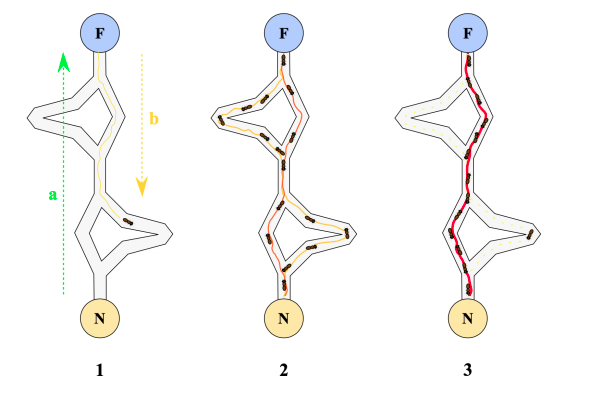
\includegraphics[width=0.9\textwidth]{ant.png}
		\caption{Работа муравьиной колонии}
		\label{ref:img1}}
\end{figure}

Процесс поиска кратчайшего пути от колонии до источника питания (рис \ref{ref:img1}):

\begin{enumerate}
	\item первый муравей находит источник пищи (F) любым способом (а), а затем возвращается к гнезду (N), оставив за собой тропу из феромонов (b);
	\item затем муравьи выбирают один из четырёх возможных путей, затем укрепляют его и делают привлекательным;
	\item муравьи выбирают кратчайший маршрут, так как феромоны с более длинных путей быстрее испаряются.
\end{enumerate}


Вероятность перехода из вершины i в вершину j определяется по формуле \ref{form:way}.

\begin{equation}\label{form:way}
	p_{i,j}={\frac {(\tau_{i,j}^{\alpha })(\eta_{i,j}^{\beta })}{\sum (\tau_{i,j}^{\alpha })(\eta_{i,j}^{\beta })}}
\end{equation}

где $ \tau_{i,j} - $ расстояние от города i до j;

$\eta_{i,j} - $количество феромонов на ребре ij;

$\alpha - $ параметр влияния длины пути;

$\beta - $ параметр влияния феромона.

Уровень феромона обновляется в соответствии с формулой \ref{form:eva}


\begin{equation}\label{form:eva}
	\tau_{i,j}=(1-\rho )\tau_{i,j}+\Delta \tau_{i,j},
\end{equation}

где $\rho$ - \text{доля феромона, которая испарится;}

$\tau_{i,j}$ - \text{количество феромона на дуге ij;}

$\Delta \tau_{i,j}$ - количество отложенного феромона, вычисляется по формуле \ref{form:add1}.

\begin{equation}\label{form:add1}
	\Delta \tau_{i,j}= \tau_{i,j}^0 + \tau_{i,j}^1 + ... + \tau_{i,j}^k
\end{equation}

где k - количество муравьев в вершине графа с индексами i и j.


% \section{Формализация задачи коммивояжера в терминах подхода муравьиных алгоритмов}

Описание поведения муравьев при выборе пути.

\begin{itemize}
	\item Муравьи имеют собственную «память».
	      Поскольку каждый город может быть посещён только один раз, то у каждого муравья есть список уже посещенных городов - список запретов.
	      Обозначим через $J_{ik}$ список городов, которые необходимо посетить муравью $k$, находящемуся в городе $i$.
	\item Муравьи обладают «зрением» - видимость есть эвристическое желание посетить город $j$ , если муравей находится в городе $i$.
	      Будем считать, что видимость обратно пропорциональна расстоянию между городами.
	\item Муравьи обладают «обонянием» - они могут улавливать след феромона, подтверждающий желание посетить город $j$ из города $i$ на основании опыта других муравьёв.
	      Количество феромона на ребре $(i,j)$ в момент времени $t$ обозначим через  $\tau_{i,j} (t)$.
	      % \item На этом основании мы можем сформулировать вероятностно - пропорциональное правило, определяющее вероятность перехода $k$-ого муравья из города $i$  в город $j$.
	\item Пройдя ребро $(i,j)$ , муравей откладывает на нём некоторое количество феромона, которое должно быть связано с оптимальностью сделанного выбора.
	      Пусть $T _{k} (t)$ есть маршрут, пройденный муравьем $k$ к моменту времени $t$ , $L _{k} (t)$ - длина этого маршрута, а $Q$ - параметр,
	      имеющий значение порядка длины оптимального пути. Тогда откладываемое количество феромона может быть задано формулой \ref{form:add}.

\end{itemize}



\begin{equation}\label{form:add}
	{\displaystyle \Delta \tau_{i,j}^k={\begin{cases}Q/L_{k}, & {\mbox{если k-ый мурваей прошел по ребру ij;}}\\0,&{\mbox{иначе}}\end{cases}}}
\end{equation}

где Q - количество феромона, переносимого муравьем.



\newpage

\section{Вывод}

В данном разделе были рассмотрены основополагающие материалы,
которые в дальнейшем потребуются при реализации алгоритмов для решения задачи коммивояжера.
